\section{X-ray Emission from the Filament}
\label{sec:Filament}

\begin{figure*}
    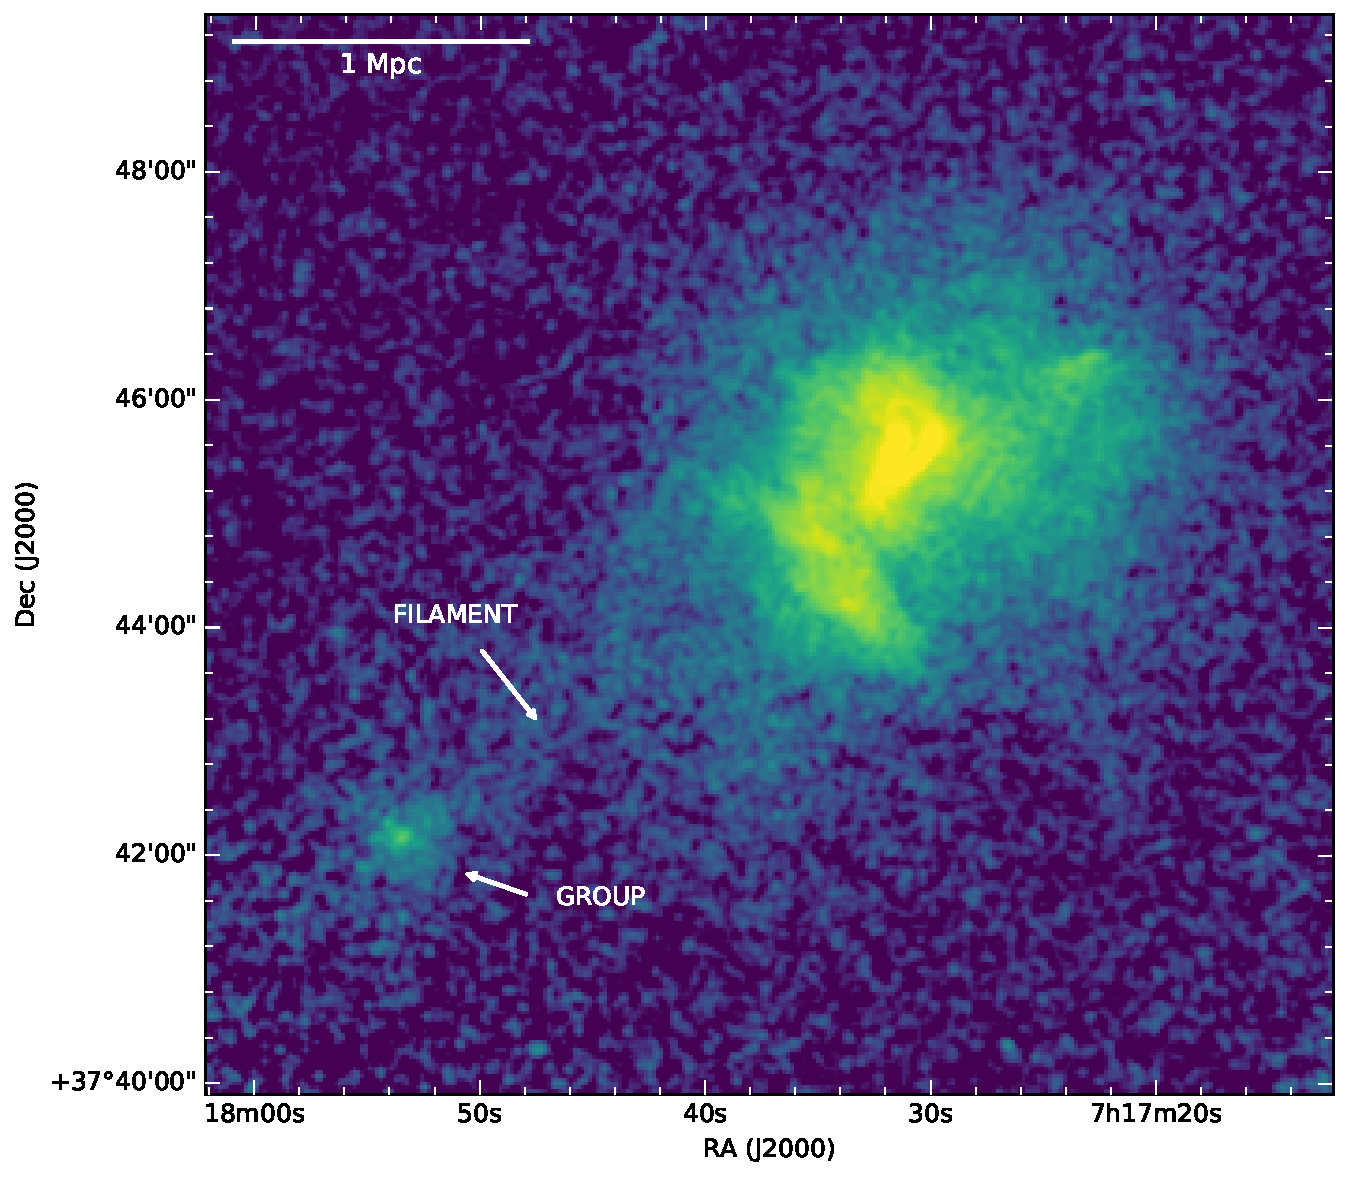
\includegraphics[width=\columnwidth]{plots/fil-labels.pdf}
    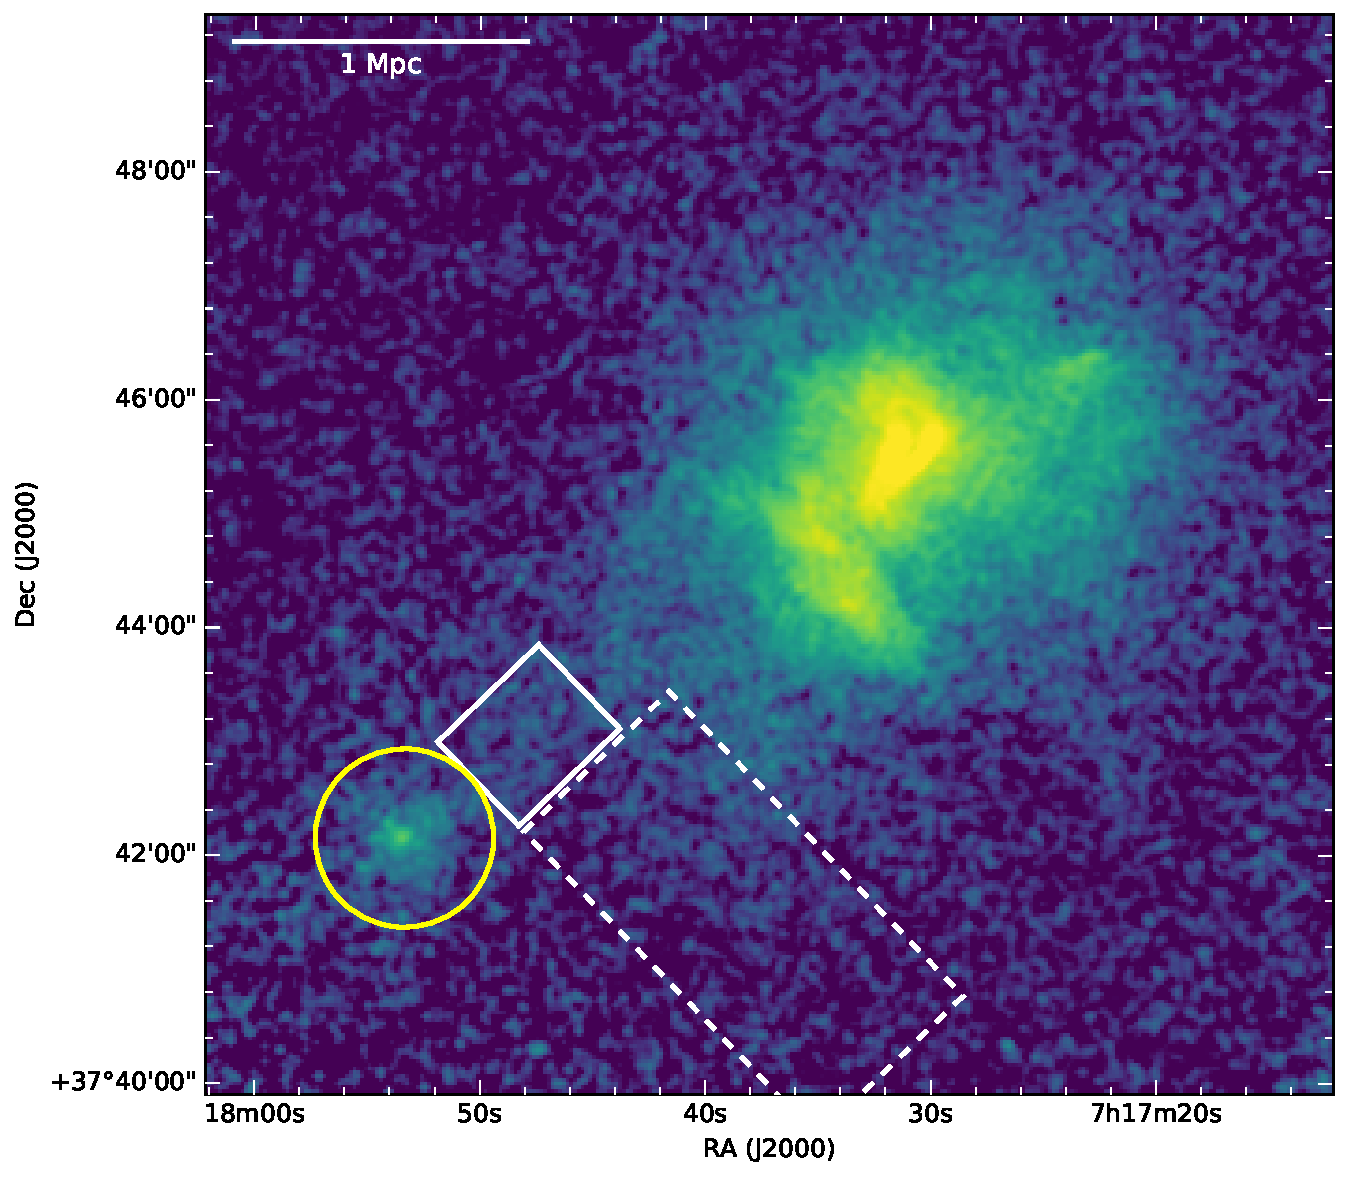
\includegraphics[width=\columnwidth]{plots/fil-regions.pdf}
    \caption{\emph{Left:} Chandra $0.5-4$~keV surface brightness map of MACS J0717.5+3745, showing the features discussed in this work. The image was exposure- and vignetting-corrected. Point sources were subtracted and the gaps were filled by sampling the regions surrounding the point sources. The gaps were filled to create a more visually appealing figure. However, the imaging analysis was done on images that did not have the gaps filled. The images used in the analysis are available online as supporting material. \emph{Right:} Regions used in the spectral analysis. The regions of main interest are drawn in solid lines, while the regions used to characterize the contaminating/surrounding emission are drawn in dashed lines. The best-fitting parameters obtained for the gas in these regions are listed in Table~\ref{tab:spectra}. \label{fig:fil}}
\end{figure*}

\begin{table}
  \caption{Parameters of the regions used for the spectral analysis. The regions are shown in Figure~\ref{fig:fil}. Uncertainties are quoted at the $\Delta C = 1$ level. \label{tab:spectra}}
  \begin{center}
    \begin{threeparttable}
      \begin{tabular}{l c c}
              \multicolumn{3}{c}{\textsc{Foreground and Background}} \\
              \hline\hline
              Model Component & Temperature\tnote{a} & Normalization\tnote{b} \\
              \hline
              Local Hot Bubble & $0.135_{-0.008}^{+0.007}$ & $7.21_{-0.18}^{+0.30} \times 10^{-7}$ \\
              Galactic Halo & $0.59_{-0.08}^{+0.09}$ & $2.78_{-0.44}^{+0.45} \times 10^{-7}$ \\
              Unresolved Background       &\multirow{2}{*}{ -- } & \multirow{2}{*}{ $4.44_{-0.37}^{+0.35} \times 10^{-7}$} \\
              Sources ObsID 16235/16305 &                                    &            \\
              Unresolved Background       &\multirow{2}{*}{ -- } & \multirow{2}{*}{ $7.02_{-0.58}^{+0.49} \times 10^{-7}$} \\
              Sources ObsID 4200               &                                    &            \\
              \multicolumn{3}{c}{} \\
              \multicolumn{3}{c}{\textsc{Large-Scale Filament}} \\
              \hline\hline
                Model Component & Temperature\tnote{a} & Normalization\tnote{b} \\
              \hline
               On Filament & $1.58_{-0.25}^{+0.51}$ & $4.00_{-0.60}^{+0.56} \times 10^{-5}$ \\
               Off Filament & $11.55_{-3.95}^{+9.09}$ & $1.55_{-0.10}^{+0.14} \times 10^{-5}$  \\
               \multicolumn{3}{c}{} \\
              \multicolumn{3}{c}{\textsc{Group in the Filament}} \\
              \hline\hline
                             & Temperature\tnote{a} & Normalization\tnote{b} \\
              \hline
                            & $4.19_{-0.48}^{+0.76}$ & $ 8.40_{-0.53}^{+0.52} \times 10^{-5}$ \\
      \end{tabular}
      \begin{tablenotes}
              \item[a] Units of keV.
              \item[b] Units of cm$^{-5}$~arcmin$^{-2}$ for the thermal components, and photons~keV$^{-1}$~cm$^{-2}$~s$^{-1}$~arcmin$^{-2}$ at 1~keV for the power-law components.
      \end{tablenotes}
    \end{threeparttable}
  \end{center}
\end{table}

To define the region of the filament that is least contaminated by ICM emission, we examined the surface brightness profile in a rectangular region aligned with the filament. In this region, the surface brightness decreases away from the cluster center, and then increases again approaching the SE group located along the filament; there is no radial range in this region where the surface brightness is flat. This suggests that the ICM of MACS~J0717.5+3745 contaminates the filament, and this contamination needs to be considered when modeling the filament emission. Alternatively, the intrinsic brightness of the filament would be decreasing towards the group; however, evidence for this scenario is weak, especially given that faint ICM emission is seen SW of the filament.

We modeled the filament and the contamination from the ICM by extracting spectra in two rectangular regions: one centered on the filament, and one positioned to the SW of it; NE of the filament, the signal-to-noise is too low for any meaningful information to be extracted from the spectrum. These regions are shown in Figure~\ref{fig:fil}. The regions were chosen to avoid the bright parts of the ICM, as well as emission from the SE galaxy group. The emission in the SW region was modeled with a single thermal component, while the emission in the filament region was modeled with two thermal components--one describing ICM contamination, whose parameters were linked to those of the thermal component used to describe the SW region, and one describing emission from the filament. The spectra from the two regions were fitted simultaneously. Table~\ref{tab:spectra} lists the best-fitting parameters obtained for a gas metallicity of 0.2 solar. Typical metallicities of cosmic filaments are still an open question, and it is plausible that they are lower than the typical metallicities in the outskirts of galaxy clusters \citep[$\sim 0.2-0.3$; e.g.][]{Simionescu2015}. In this case, varying the metallicity causes only minor changes to the best-fitting parameters, well within the statistical uncertainty ranges. In one of the \textsc{Jupyter} notebooks supporting this letter, we also list the results obtained for metallicities of 0 and 0.1 solar.\footnote{\url{https://goo.gl/e8xQD0}}

The \textsc{XSpec} normalizations of the thermal components listed in Table~\ref{tab:spectra} are defined as
\begin{equation}
	\mathcal{N} = \frac{n_{\rm e} \, n_{\rm H} \, V}{10^{14} \, 4\pi \, S_{\rm reg} \, D_{\rm A}^2 \, (1+z)^2} \, , 
\label{eq:norm}
\end{equation}
where we assume the density to be constant in each region, where $n_{\rm e}$ is the electron number density, $n_{\rm H}$ is the hydrogen number density, $V$ is the volume of the region, $S_{\rm reg}$ is the projected area of the region, $D_{\rm A}$ is the angular size distance to the cluster, and $z$ is the cluster redshift.

\begin{figure}
	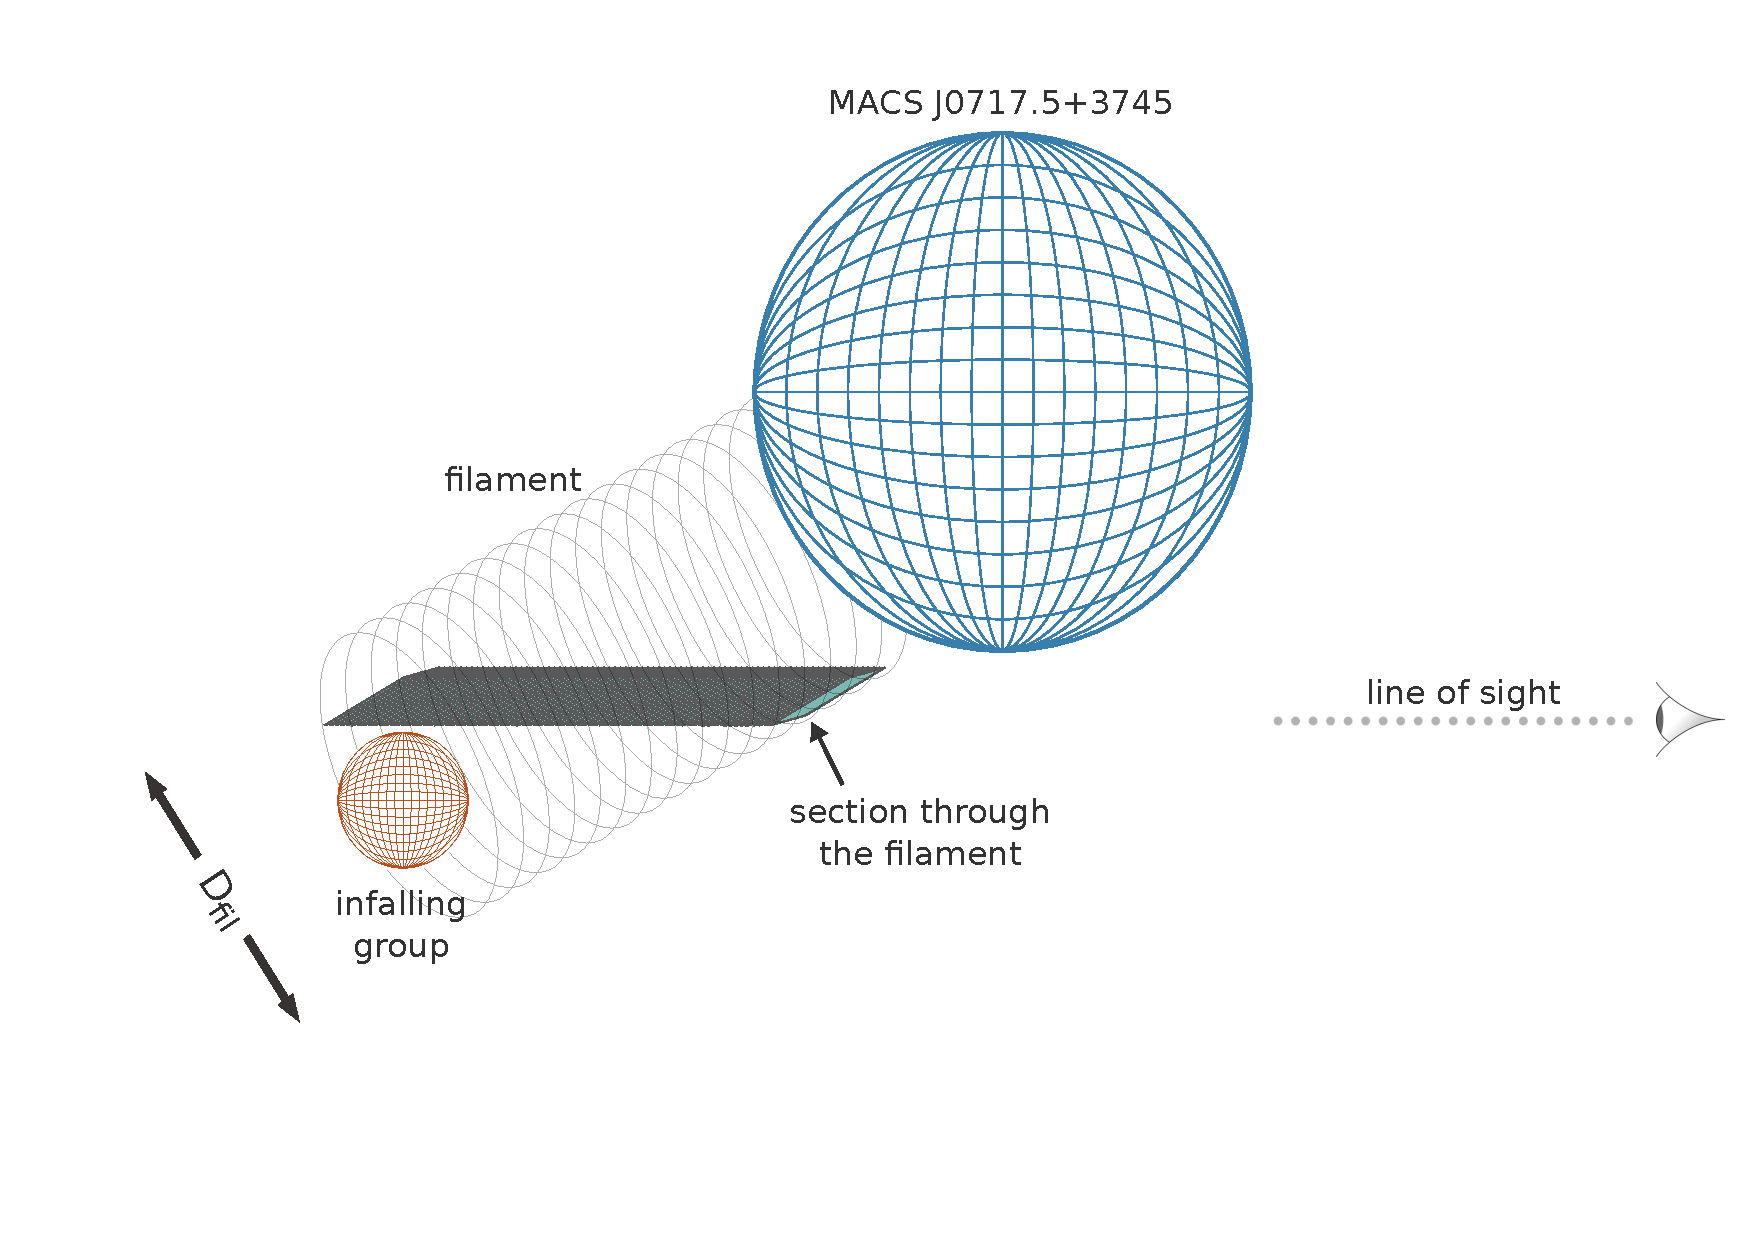
\includegraphics[width=\columnwidth, trim=0 2.5cm 0 1cm, clip=True]{plots/fil-macsj0717-sketch.pdf}
	\caption{Sketch illustrating the geometry assumed for the large scale filament. The results vary insignificantly (compared to our other uncertainties) when assuming a parallelepiped geometry instead of a more natural cylindrical shape. For simplicity, we therefore used a parallelepiped for our volume estimate. The parallelepiped has two rectangular faces perpendicular to the line of sight, and two rectangular and two parallelogram faces parallel to the line of sight. The normal to the parallelogram faces points perpendicular to the page.  \label{fig:sketch}}
\end{figure}

To calculate the density of the filament in the region shown in Figure~\ref{fig:fil}, we assumed that in 3D the region is a parallelepiped with two rectangular faces perpendicular to the line of sight, and two rectangular and two parallelogram faces parallel to the line of sight. A sketch of this 3D section through the filament is shown in Figure~\ref{fig:sketch}. \citet{Jauzac2012}, citing Ebeling et al., in prep., quoted a filament inclination angle $\theta \sim 75$ degrees with respect to the plane of the sky (the results below are highly sensitive to the uncertainty on the inclination angle). They also determined the filament has a diameter $D_{\rm fil} \sim 3$~Mpc at the radius from which our spectra were extracted. Therefore, the volume of the parallelepiped corresponding to our region equals the filament diameter times the area of the parallelepiped face seen along the line of sight, i.e.
\begin{eqnarray}
    V \equiv V_{\rm ppp} = D_{\rm fil} \; S_{\rm reg} / \cos\theta\,  , 
\label{eq:v_ppp}
\end{eqnarray}

The projected region has a length of $1.2$~arcmin ($\approx 460$~kpc) and a width of $1$~arcmin ($\approx 380$~kpc), therefore $S_{\rm reg} = 1.2$~arcmin$^{2}$. Assuming $n_{\rm e} = 1.2\, n_{\rm H}$ \citep[e.g.,][]{Bohringer2010}, and finally substituting Eq.~\ref{eq:v_ppp} in Eq.~\ref{eq:norm}, the electron number density in the X-ray bright part of the filament is $\sim 2\times 10^{-4}$~cm$^{-3}$. The critical density of the Universe at the redshift of MACS~J0717.5+3745 is $1.7\times 10^{-29}$~g~cm$^{-3}$. Assuming the total baryon density is $4.4\%$ the critical density of the Universe \citep{Kirkman2003}, the filament is overdense by a factor of $\sim 450$ compared to the mean baryon density of the Universe. Assuming a baryon mass fraction of $0.15$ \citep[e.g.,][]{Mantz2014}, the mass density of the filament is $\sim 3\times 10^{13}$~M$_{\odot}$~Mpc$^{-3}$. The filament density is therefore in excellent agreement with the density calculated from the weak lensing data by \citet{Jauzac2012} for the same filament geometry. The filament density corresponds to an overdensity of $\sim 100-150$ relative to the critical density of the Universe.\footnote{\citet{Jauzac2012} calculate an overdensity of $206\pm 46$~$\rho_{\rm crit}$, about $65\%$ higher than our value, but this appears to be due to a mistake in the density conversion; our filament mass density values are consistent.} 

The X-ray emission from the brightest part of the filament could originate from the hottest gas phase of the WHIM. Its density and temperature are consistent with reports of WHIM X-ray detection from other cluster filaments \citep[e.g.,][]{Werner2008, Eckert2015}. Alternatively, at least part of the X-ray emission could be due to gas stripped from substructure that fell onto the cluster along the large-scale filament. However, the latter interpretation requires that the X-ray-bright part of the filament is within the virial radius of MACS~J0717.5+3745 \citep[$r_{\rm 138} = 2.5$~Mpc;][]{Medezinski2013}, which would imply a filament inclination angle of $\lesssim 60^\circ$. 

For the densities calculated above, the mass of the filament in the region from which the spectra were extracted is $\sim 6\times 10^{13}$~M$_\odot$, with $\sim 9\times 10^{12}$~M$_\odot$ in the hot gas. 

\begin{figure*}
   \renewcommand{\arraystretch}{1.5}
    \begin{tabular}{m{\columnwidth}m{0.9\columnwidth}}
    \multicolumn{2}{l}{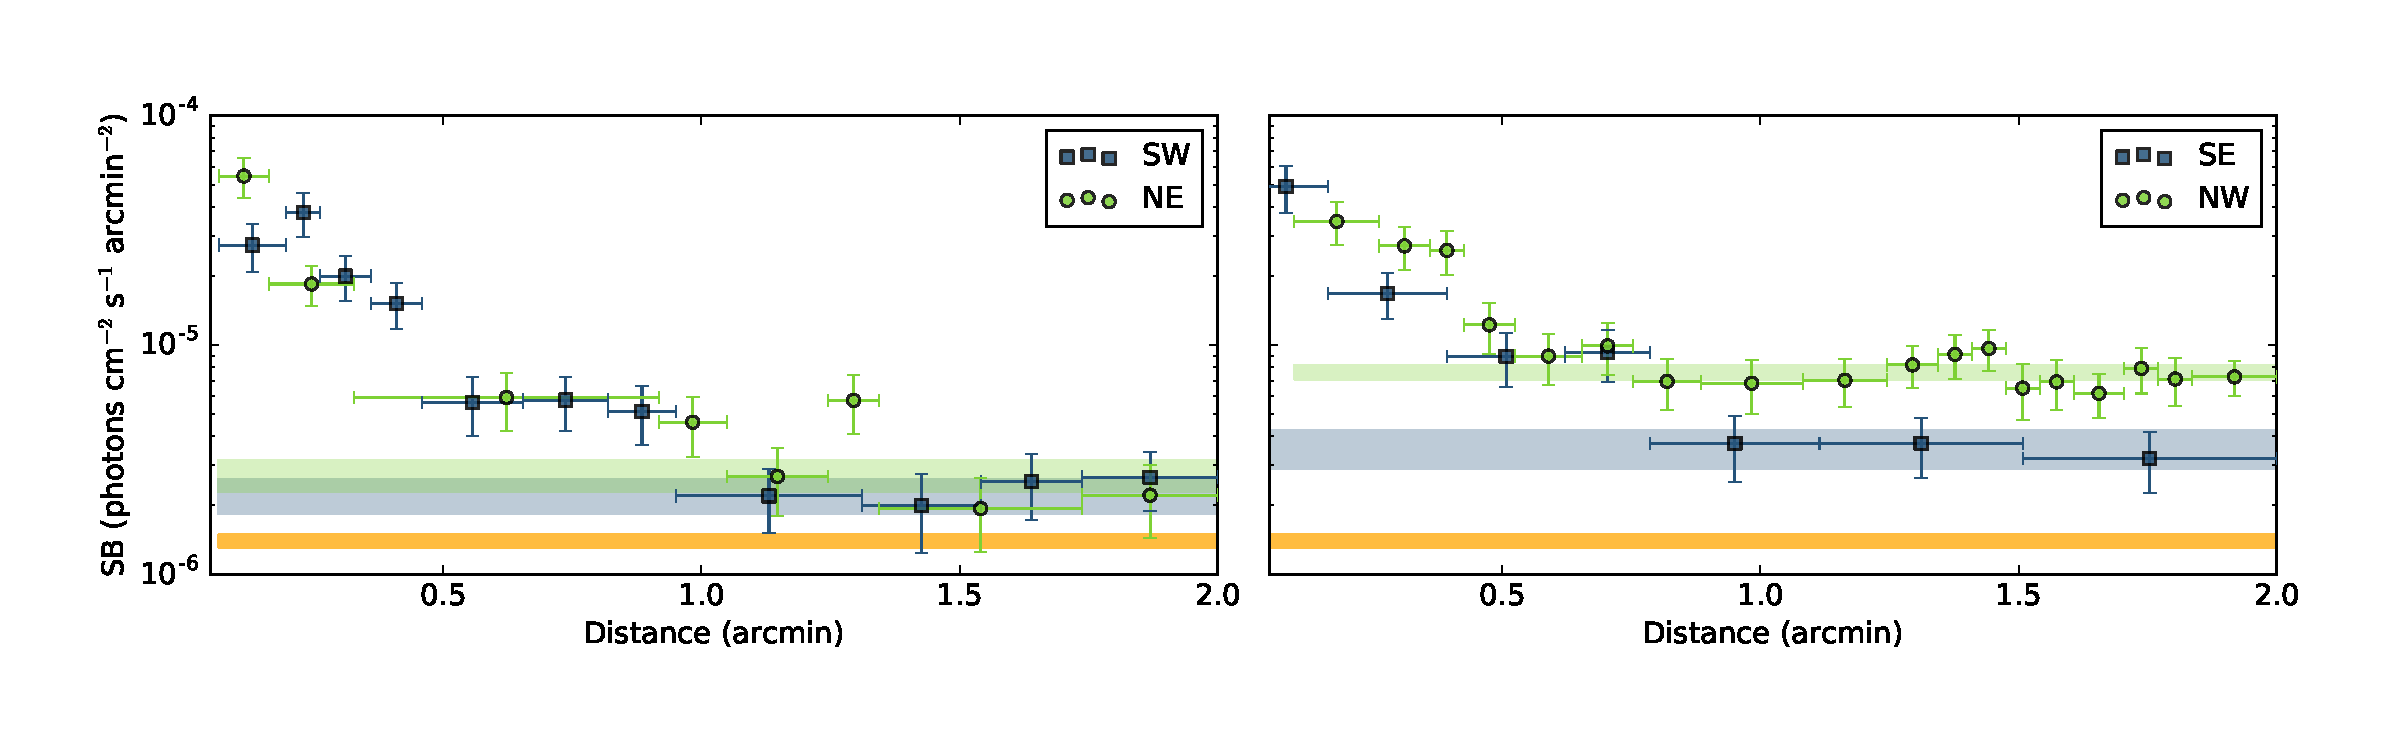
\includegraphics[width=\textwidth]{plots/macsj0717-group-all-directions.pdf}} \vspace{-0.5cm} \\
    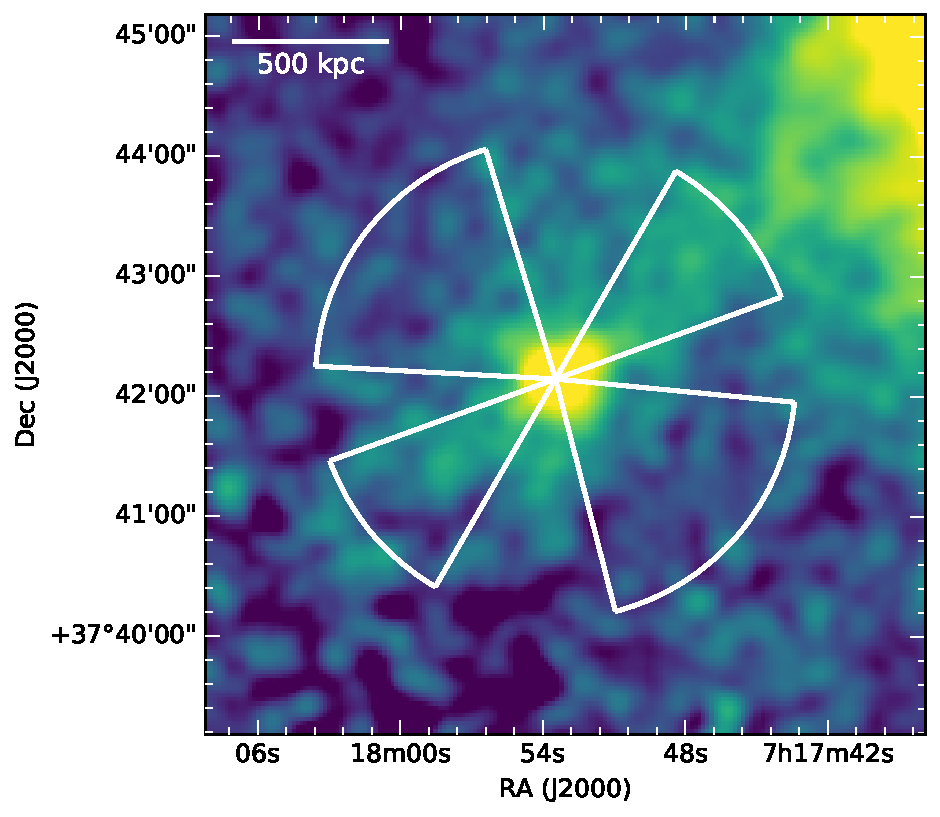
\includegraphics[width=\columnwidth]{plots/group-sectors.pdf}
    & \hspace{0.15cm}\multicolumn{1}{b{0.85\columnwidth}}{\caption{\emph{Top:} Surface brightness profiles perpendicular to (left) and along (right) the filament. The light-colored green and blue bands show the average surface brightness between 1 and 2 arcmin, where the emission from the group is negligible. The orange band shows the $1\sigma$ confidence range of the sky background level. \emph{Bottom:} Sectors from which the surface brightness profiles shown above were extracted. The sectors are centered on the X-ray peak of the galaxy group. }} 
    \label{fig:group-sx}
    \end{tabular}
\end{figure*}

In Figure~\ref{fig:group-sx}, we show the surface brightness profiles in four sectors centered on the galaxy group seen within the filament. The surface brightness of the group becomes negligible beyond 1 arcmin. Between 1 and 2 arcmin, the profiles show the NW sector being significantly brighter than the other three; this sector covers the part of the filament between the group and the cluster. On the other side of the group, in the SE sector, the surface brightness between 1 and 2 arcmin is also larger than in the directions perpendicular to the filament. The SE sector includes part of the filament at higher cluster-centric radii. The surface brightness here is about half of that in the NW sector, which implies a baryon density lower by a factor of $\sim 1.5$ compared to the part of the filament closer to the cluster if the diameter of the filament is the same on both sides of the group. However, \citet{Jauzac2012} found that the diameter of the filament might be decreasing by a factor of up to $\sim 2$ from the region ahead of the group to the region beyond the group. Bearing in mind that the measurements of \citet{Jauzac2012} are highly uncertain, the decrease in diameter could account for the difference in surface brightness with no decrease in the baryon density of the filament.

The calculations made above can be found in one of the supporting \textsc{Jupyter} notebooks accompanying this paper.\footnote{\url{https://goo.gl/eQbTYd}}





